\documentclass[12pt, a4paper]{scrartcl}
\usepackage[utf8]{inputenc}
\usepackage{amsmath}
\usepackage{mathpazo}
\usepackage[margin=1in]{geometry}
\usepackage{setspace}
\usepackage[T1]{fontenc}
\usepackage[utf8]{inputenc}
\usepackage{scrlayer-scrpage}
\usepackage[usenames,dvipsnames]{xcolor}
\usepackage{easyReview}
\usepackage[numbers,sort&compress]{natbib}
\usepackage{hyperref}

\title{Comparison of Multi-Response Estimation Methods}
\subtitle{Reviewers Comments}
\author{\vspace{-5ex}}
\date{\vspace{-5ex}}

\automark*[subsection]{section}
\chead*{}
\ohead*{Comparison of Multi-Response Estimation Methods}
\ihead*{Reviewers Comments}
\ofoot*{{\headmark} $\vert$ \pagemark}
\cfoot*{}

\setlength {\marginparwidth }{2cm}
\setstretch{1.25}
\setkomafont{disposition}{\normalfont\bfseries}
\setcounter{secnumdepth}{0}
\colorlet{mycolor1}{NavyBlue}
\colorlet{mycolor2}{Violet}
\colorlet{critical}{RedOrange}
\colorlet{good}{ForestGreen}
\colorlet{info}{OliveGreen}
\colorlet{answers}{PineGreen}

\setlength{\parindent}{0pt}
\setlength{\parskip}{12pt}

\makeatletter
\DeclareOldFontCommand{\rm}{\normalfont\rmfamily}{\mathrm}
\DeclareOldFontCommand{\sf}{\normalfont\sffamily}{\mathsf}
\DeclareOldFontCommand{\tt}{\normalfont\ttfamily}{\mathtt}
\DeclareOldFontCommand{\bf}{\normalfont\bfseries}{\mathbf}
\DeclareOldFontCommand{\it}{\normalfont\itshape}{\mathit}
\DeclareOldFontCommand{\sl}{\normalfont\slshape}{\@nomath\sl}
\DeclareOldFontCommand{\sc}{\normalfont\scshape}{\@nomath\sc}
\makeatother

\begin{document}

\maketitle

\section{Reviewer One}

This manuscript compared the parameter estimation accuracy of some Multi-response linear regression model by simulated data with varying properties. This work gave some insights into these methods and helped the researchers to understand their performance. Based on this point, this work obtained some findings. I have the following comments and questions on this manuscript which the authors should consider.

\begin{itemize}
    
\item Some authors' name should be corrected, for example, N{\ae}s on Page 3.

\textcolor{gray}{Fix Names in the references: Double Names, Norwegian Characters and remove months.}
\textcolor{answers}{All Fixed.}

\item I think the writing about the scalar, vector, and matrix should be used according to the general rule. For example, italic lowercase is used for scalar, such as equations (9) and (10).

\textcolor{gray}{Writing the equation in proper mathematical form/notation requires introduction of new symbols. So, we can say that the equation is a heuristic representation and the term in the brackets represents the effect of corresponding simulation parameters. The cubic notation represents the third order interaction of these effects. $\boldsymbol{\mu}$ in both equations are different so I will change it to $\mu_{u_j}$ and $\mu_{v_j}$ with corresponding update in the response vector $\mathbf{u}$ and $\mathbf{v}$ and rewrite them as $(u_j)$ and $(v_j)$ where $j=1, \ldots m$ responses.}

\textcolor{mycolor1}{\textbf{Changes: \textit{First paragraph in Analysis section}}}\hfill \\
    \textcolor{answers}{Here the equations represent a heuristic representation of the MANOVA model and is closer to R-representation than a proper mathematical formulation. In the model, we will consider up-to the third order interaction of simulation parameters (\texttt{p}, \texttt{gamma}, \texttt{eta}, and \texttt{relpos}) and \texttt{Method} as is represented by cube notation.}

\item Please explain why the optimal components determined in these methods are different. I hope the authors could give further explanation about this.

\textcolor{gray}{We can write that envelopes are the linear components of relevant eigenvectors. As it is further compressed, it is usual that the method uses fewer number of components than that of others. In the case of PLS, as it uses covariance between the predictors and responses to identify its coefficients, it uses fewer number of components than PCR, especially in the case when relevant components are further away.}

\textcolor{mycolor1}{\textbf{Changes: \textit{Last paragraph of estimation methods section and just above the experimenal design section}}} \hfill \\
\textcolor{answers}{
... have discussed when and under which condition the population models of PCR, PLS and Xenv are equivalent. \\\\
Here, each methods uses different strategy for estimating the regression coefficients, the optimal number of components they determine will be different. For example, PCR method captures the maximum variation in predictor matrix in every subsequent components while PLS methods focus more on the variation in predictors that are relevant for the responses. The envelope methods construct the envelope as a linear combination of relevant eigenvectors. This allows them to reduce the dimension even further and consequently these methods have smaller optimal dimension.
}

\item Please show the relationships of the relevant space form the compared methods. I hope the authors could give further discussion about this.

\textcolor{gray}{I think this is the part Inge Paper has discussed in details.}

\textcolor{answers}{The above answer and the reference to the Inge Helland Paper 2016.}

\item For the real data, I think the manuscript has a significant flaw that don't use a real data to validate the parameter estimation accuracy of compared methods. It is of a prime importance to used real dataset to help readers of Chemo-lab to understand the method. Thus, it is strongly recommended the authors apply at least one real dataset to show their performance.

\textcolor{mycolor1}{We need to find some data that also has a basis of calculating the true relationship. An alternative suggested by Trygve is to find a data with large number of observations and the estimation from the complete set can be regarded as a true beta and just use subset of observation for the comparison.}

\textcolor{critical}{Have not found a proper data yet. But will try to use two dataset I have even if they do not have enough observations.}

\item The GitHub repository is not available, an applicable version should be provided.

\textcolor{answers}{It is working. See: \href{https://github.com/therimalaya/04-estimation-comparison}{
\textcolor{mycolor1}{\texttt{https://github.com/therimalaya/04-estimation-comparison}}} in the last sentence.}

\end{itemize}

This paper gives an elaborate organisation that is very helpful for reading. This is commendable.

\section{Reviewer Two}

This paper is a followup to an earlier paper on multi-response prediction methods by the same authors. Accordingly, I had to read the prediction paper before turning to the current submission on estimation. I initially expected the estimation results to largely parallel those for prediction, but it turned out that there were a few surprises, particularly the behaviour of envelope estimation in the presence of highly correlated responses, as represented in Table 1. One possible explanation for this phenomenon comes to mind. \textcolor{gray}{The log likelihood objective functions for envelope methods are non convex. It seems possible, depending on the sample size, that highly correlated responses produce objective functions with multiple maxima of not substantially dissimilar magnitudes.} \textcolor{answers}{This is the exact reason, in equation 5 and equation below 6, we have used the variance of each response to scale the estimation error which will lessen this differences.} If so, it may be possible for the algorithms to get caught at a local point relatively far from the true value. This might also explain the predictive performance of envelopes. Multiple local optimal of not dissimilar magnitudes means that the data support multiple values for $\beta$, which translates in terms of the likelihood into similar predictions. \textcolor{gray}{This might be tested by running the algorithms at different starting values, including one at the true value of the regression coefficients.} \textcolor{answers}{Although this might be tested, this is out of scope of this study. Since we are more focused on comparison different methods rather than evaluating the properties of envelope methods. In addition, the estimation errors are scaled by the variance of the responses of dissimilar magnitudes, this should somewhat adjust the effect of such variation although not entirely.} Here Xenv might be sufficient since its performance in Table 1 is similar to that of Senv. Another possibility is to plot the objective functions along selected directions. \textcolor{gray}{This additional effort would seem necessary to (hopefully) explain one way in which the submission diverges from the results in the previous paper.} \textcolor{answers}{Yes, it is necessary to explain for the departure of the results from prediction paper which has been discussed in "Discussion and Conclusion" Section second last paragraph, however, this study tries to give similar weight and comparison to all the methods and is not able to study envelope methods and their particular properties in a particular case.}

\textcolor{answers}{In this study, we have fixed the number of observation at 100 and a comparison is made on different methods. Although not included in the analysis, In the following figure, we have tried to compare how the estimation error decrease in these methods when the number of observation changes. The figure shows a significant decrease in estimation error for all methods.}

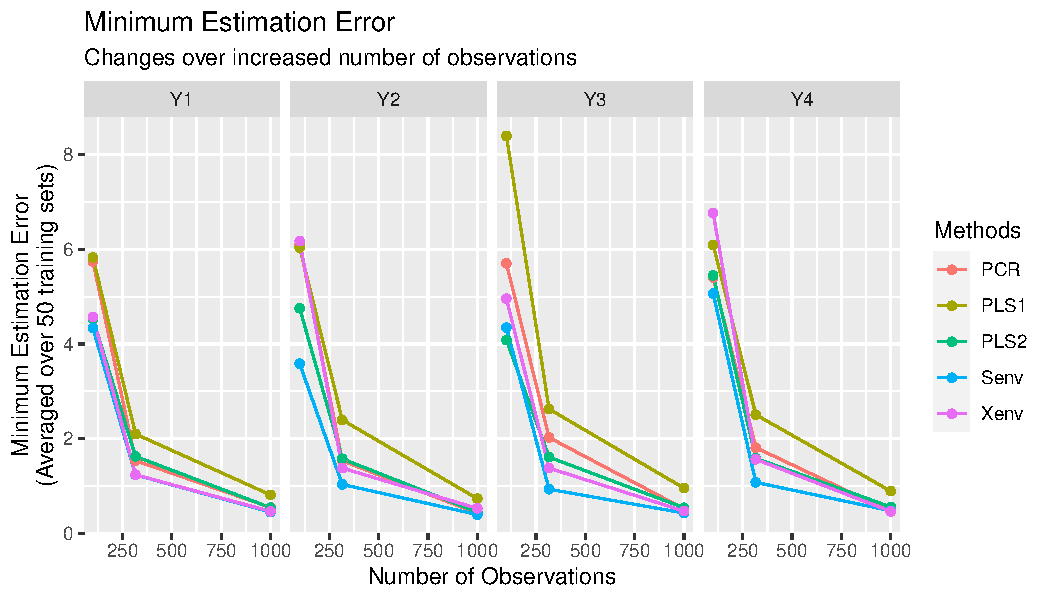
\includegraphics[width=\textwidth]{n-vs-est-err.pdf}

Another of my general reactions is that the clarity of presentation needs attention. \textcolor{gray}{There seem to be simulation details missing and some statements are not sufficiently clear.} 

\textcolor{answers}{\textcolor{mycolor1}{\textbf{In the paragraph of \textit{Position of relevant Components} (Around Page 7): }}\\
Here we will use two different levels of a position index of true predictor components ...}. 

\textcolor{gray}{A quibble:
I prefer indented paragraphs, as the current style sometimes makes it unnecessarily hard to tell the start of a paragraph, which is annoying.}

\textcolor{answers}{Fixed now.}

\textit{Top of page 6}: PCR cannot be equivalent to PLS and Xenv under the definition of PCR given on the bottom of page 4. Helland must have been using a different notion of PCR.

\textcolor{answers}{\textcolor{answers}{... have discussed when and under which condition the population models of PCR, PLS and Xenv are equivalent.}}

\textit{Page 6, sample size}: The envelope methods, being based on the likelihood, are asymptotically efficient and so, with n sufficiently large, must do better than the other methods in both
estimation and prediction. This might be mentioned for completeness.

\textcolor{gray}{I think this is the part we can mention. This also gives some difference/similarity between prediction and estimation in the case of small/large sample size.}

\textcolor{critical}{
\textbf{\textcolor{mycolor1}{\textit{End of second paragraph of discussion and conclusion section}}} \hfill\\
Since the envelope methods are likelihood based and are asymptotically efficient (ref ....), with sufficiently large number of samples, the methods can produce smaller prediction and estimation errors than others usual MLE methods.}
\begin{verbatim}
- Here does the asymptotically efficient refers to smaller prediction 
  and estimation errors?
- When I went through some literature, it is efficient than usual MLE 
  methods, does this apply for PLS1 and PLS2 as well. What about the 
  interaction of efficiency with the biasedness?
\end{verbatim}

\textcolor{answers}{Here I have also tried to see how envelope methods behave when large number of observation is used $n>>p$. Following figure gives an idea for design 29 when $n=10000$ is used.}

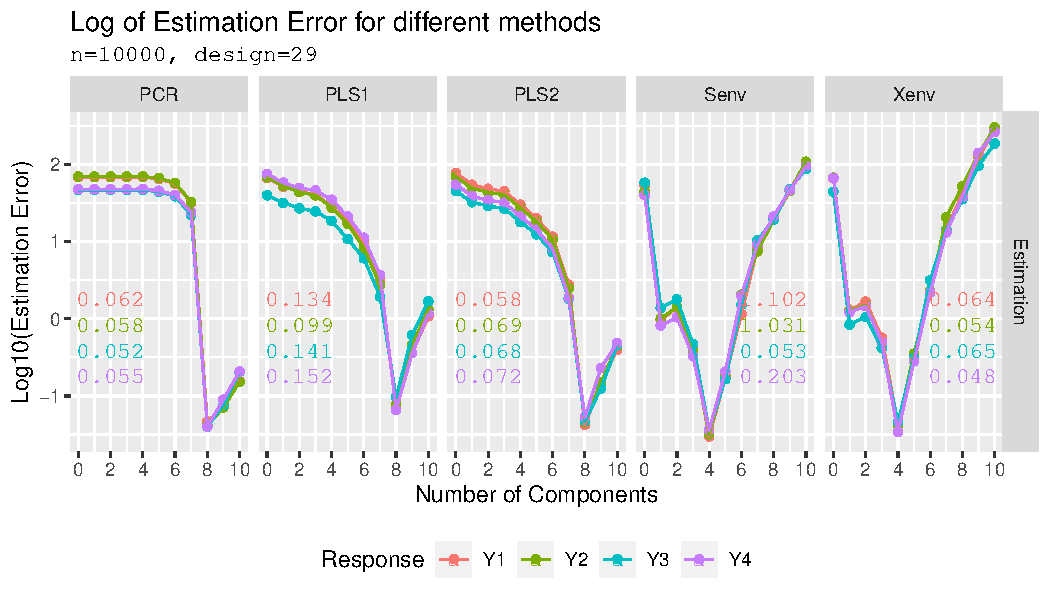
\includegraphics[width=\textwidth]{large-n-est-error.pdf}

\textit{Section 4. Experimental Design}: The description of the experimental design should enable
the reader to reconstruct the model as given in (1) and (2), but that does not now seem
possible. How were $\Sigma_{yy}$, $\Sigma_{yx}$ and $\Sigma_{xx}$ constructed, as the eigenvalues are only part of the story? It’s my understanding that the columns of $\beta$ can be written as linear combinations of either eigenvectors 1,2,3,4 or 5,6,7,8 of $\Sigma_{xx}$. How was this accomplished? If $\beta$ is full column rank then it seems that the true number of components must be 4.

\textcolor{gray}{Here we can mention about the random rotation matrix we have constructed based on the relevant predictor user wants as a simulation parameters. Although the true components will be 4 in both cases, all predictors are somewhat relevant and shares the same information space as the four true components.}

\textcolor{answers}{
\textcolor{mycolor1}{\textbf{\textit{Experimental Design:} First paragraph}}\hfill \\
... In the simulation, number of response variables $m = 4$ and number of observations $n = 100$ are fixed, and the ...}

\textcolor{answers}{
\textcolor{mycolor1}{\textbf{\textit{Experimental Design:} After the discussion of simulation parameters}}\hfill \\
Using these simulation parameters, a latent covariance matrix is constructed as in 5.
\begin{equation*}
  \begin{bmatrix}
    \mathbf{w} \\ \mathbf{z}
  \end{bmatrix} 
  \sim \mathsf{N}
  \begin{pmatrix}
    \begin{bmatrix}
      \boldsymbol{\mu}_w \\
      \boldsymbol{\mu}_z \\
    \end{bmatrix}, &&
    \begin{bmatrix}
      \boldsymbol{\Sigma}_{ww} & \boldsymbol{\Sigma}_{wz} \\
      \boldsymbol{\Sigma}_{zw} & \boldsymbol{\Sigma}_{zz} 
    \end{bmatrix}
  \end{pmatrix}
\end{equation*}
For example, $\eta=1.2$ gives $\boldsymbol{\Sigma}_{ww}$ as a diagonal matrix with 1, 0.3, 0.09, 0.03 in its diagonal. However, for $\eta=0$ it will be an identity matrix $\mathbf{I}_4$. A similar approach is used for covariance matrix $\boldsymbol{\Sigma}_{zz}$. In addition, when the true relevant components are at position 1, 2, 3, 4, the covariance matrix $\boldsymbol{\Sigma}_{wz}$ with dimension $p \times m$ will have $\sigma_{11}, \sigma_{12}, \sigma_{13}$ and $\sigma_{14}$ in its first four columns and the rest are filled with zeros. These $\sigma$ values are the links that defines the relationship between the latent components of predictors and the first response component. A random orthogonal rotation matrix $\mathbf{R}$ and $\mathbf{Q}$ are used to rotate these latent covariances in order to obtain covariance matrices in 1. Rimal et al. (2018) have discussed the underlying mechanism in details.
}

It is stated on page 7 that simulations were restricted to regressions with only one response component. How was this component constructed? Was the number of predictor components also restricted by the simulation? If so, how? This seems important because of the different numbers of components selected by the various methods as represented in Figure 7. Naturally one wonders about the true number of components set in the simulation.

\textcolor{gray}{Here as well, we should refer to the Simrel-M paper and summarise that the covariance matrix we constructed is actually between the latent components which were later rotated together with additional normally distributed random vectors.}

\textcolor{answers}{The above answer will also settle this issue.}

The page 7 sentence ``In the final dataset all predictors together span the same space as the relevant predictor components $\ldots$'' makes no sense to me since all predictors together should span $\mathbb{R}^p$, unless $\Sigma_{xx}$ is singular.

\textcolor{gray}{I think we need to make this clear as it is not the same space but the information space. In other words, the $p$ predictors contains the same information relevant for the response that is also contained in the four relevant components.}

\textcolor{answers}{Here we have assumed that there is only one informative response component. ... In the final dataset all predictors together span the same \textbf{information} space as the relevant predictor components and all responses together span the same \textbf{information} space as the one informative response component. ...}

\textcolor{gray}{Page 8, line 5 from the bottom: Figure ??} \textcolor{answers}{Fixed}

\textit{Section 5. Basis of Comparison}: I’m a bit perplexed by the choice of the inner product matrix in (5). Since the eigenvalues of $\Sigma_{xx}$ are different, the predictor variances differ, unless $\Sigma_{xx}$ was constructed as a constant times a correlation matrix. And the predictors are of course correlated. The columns of $\beta$ were scaled by the response variances but there was evidently no effort to correct for the different variances or correlations of the predictors. In view of what I know about the simulation setup, I would have thought that $\Sigma_{xx}$, instead of the identity, is a more appropriate inner product. A case can also be made for using $\Sigma_{xx}^{-1}$ as the inner product, but I can’t see any clear justification for using the identity.

\textcolor{gray}{Including $\Sigma_{xx}$ in estimation error expression makes no sense. Aren't we trying to see how different the estimated coefficients are from true? When we include the data that was used to estimate the coefficient also to calculate the error, aren't we influencing the error using the error itself.}

\textcolor{answers}{Since, the expression is the squared difference of estimated regression coefficient from the true coefficients which is fair measurement of the estimation error. Using $\Sigma_{xx}^{-1}$ will rescale and influence the difference of these estimates from their truth with the data that is used to estimate them.}

\textcolor{critical}{Not sure if the above answer will be sufficient since the reviewer is concern about why scaling with response variance not with predictor variance? I feel that we should give some extra explanation here.}

\textit{Section 6. Exploration}:. Figure 4 is difficult to interpret because one needs to take careful note of the scales for the $\gamma = 0.2$ and $\gamma = 0.9$ plots. At $\gamma = 0.9$ I can’t see any obvious differences in the methods. The claim that ``$\ldots$ envelope methods tend to have increased estimation error in cases of highly correlated responses (eta: 1.2), whereas $\ldots$'' may be true,
but I can’t see it from the figure. In particular, I can’t see that any method is “best” at $\gamma = 0.9$ and $\eta = 1.2$. The plot does clearly show the impact of relative position.

\textcolor{gray}{Either we need to change our view and remove this or we can add that the conclusion is for the relative comparison of envelope methods with others in these two cases. So, this can not be taken as wrong-doing of envelope rather we are saying that the it is less able to be very good in the second case.}

\textcolor{answers}{We have removed the last sentence of the paragraph. I think the reviewer is correct. It is difficult to see the difference from the figure alone.}

Might the relatively large number of components for PCR, PLS1 and PLS2, shown in Figure 5 partly explain their relatively poor performance in the previous paper? When reading the top of page 13, I again found myself wondering about the true number of components.

\textcolor{gray}{This will be fixed by the previous fix.}

\textcolor{answers}{Fix in Experimental design section will settle this issue.}

The conclusion in the penultimate sentence on page 13 evidently comes from Table 1. But Figure 6 shows that envelopes do well in estimation with one component and no evident bias, while PLS2 needs 7 or 8 components to give the same visual impression. I would have thought that the estimation variation increases with the number of components, so PLS2 estimators would be noticeably more variable than envelope estimators. Is this reflected in the simulations somehow, or is my intuition wrong?

\textcolor{gray}{Is he talking about the variablility in estimation error between different replicates or between different number of components. In the seconds case, PLS has shown the variability when large number of components are included in some cases but not as in envelope methods. Since the envelope are based in MLE, the variability raise sharply especially when $p$ approaches $n$.}

\textcolor{answers}{In that particular case with design 9 and 29, the true predictor components are at position 5, 6, 7, 8. In PLS2, its estimation error gets its minimum only after including 7-8 number of components in their model while envelope methods, minimum errors are obtained in either first or second component. If we include more than 8 components in PLS or PCR methods, the estimation error in their case also starts increasing we can see in figure 7. The paragraph mentioned here is just to state this observation.}

\textcolor{answers}{
\textcolor{mycolor1}{\textbf{\textit{Following paragraph is added at the end of paragraph mentioned by the reviewer}}} \hfill \\
Here, the variation in the estimation error can increase drastically also for PCR and PLS methods, when number of components more than 10 (not seen in the figure) is included. This is hinted in the estimation error plot (Figure 7) for PLS2 for 8-10 number of components are included in the model.}

In the first full sentence on page 15, to what does “Here the . . . ” refer. All of section 6? Just the material following the paragraph?

\textcolor{gray}{I will replace Here with concrete statement or refer to a figure.}

\textcolor{answers}{I have replace "Here" in two places,
\begin{itemize}
    \item \textcolor{mycolor1}{\textbf{\textit{Second last paragraph of exploration section:}}}\\ \textit{In the figure}, PLS2 ...
    \item \textcolor{mycolor1}{\textbf{\textit{Second last paragraph of page 14}}}\\ \textit{In this study}, the ...
\end{itemize}}

Last sentence in third full paragraph on page 15 ``However, one should $\ldots$'' and sentence ``However, non-optimal number $\ldots$'' starting on line 6 from the bottom on page 22: My guess is that these statements come from the estimative performance of Senv in Figure 7 for 7–10 components. The conclusion is then based on comparing Senv at > 5 components above its optimum number of components to PLS2 at < 3 components above its optimum. To be on a equal footing, shouldn’t these methods be compared at the same number of components above the optimum?

\textcolor{gray}{Here, aren't we talking about choosing right number of components when working with real dataset rather than in this simulation?}

\textcolor{answers}{\textcolor{mycolor1}{\textbf{\textit{The sentence referred by the reviewer:}}} \hfill \\
However, one should be cautious about determining the optimal number of components using method like cross-validation while working with real data.}

\textcolor{answers}{\textcolor{mycolor1}{\textbf{\textit{Also mentioned in third last paragraph}}} \hfill \\
careful in this respect while using the envelope methods which can easily be controlled through a method like cross-validation.}

\textit{Section 7. Analysis:} Nice discussion.

\textcolor{answers}{Thank you}

\section{Extra Stuffs}
\begin{cbox}{black}{gray!10}
\small
\textcolor{gray}{I think this is the part we can mention. This also gives some difference/similarity between prediction and estimation in the case of small/large sample size.}

\textcolor{critical}{
\textbf{\textcolor{mycolor1}{\textit{End of second paragraph of discussion and conclusion section}}} \hfill\\
Since the envelope methods are likelihood based and are asymptotically efficient (ref ....), with sufficiently large number of samples, the methods can produce smaller prediction and estimation errors than others usual MLE methods.}

\begin{itemize}[leftmargin=1em]
\item Here does the asymptotically efficient refers to smaller prediction 
  and estimation errors?
\item When I went through some literature, it is efficient than usual MLE 
  methods, does this apply for PLS1 and PLS2 as well. What about the 
  interaction of efficiency with the biasedness?
\end{itemize}

\textcolor{answers}{Here I have also tried to see how envelope methods behave when large number of observation is used $n>>p$. Following figure gives an idea for design 29 when $n=10000$ is used.}

\vspace{1em}

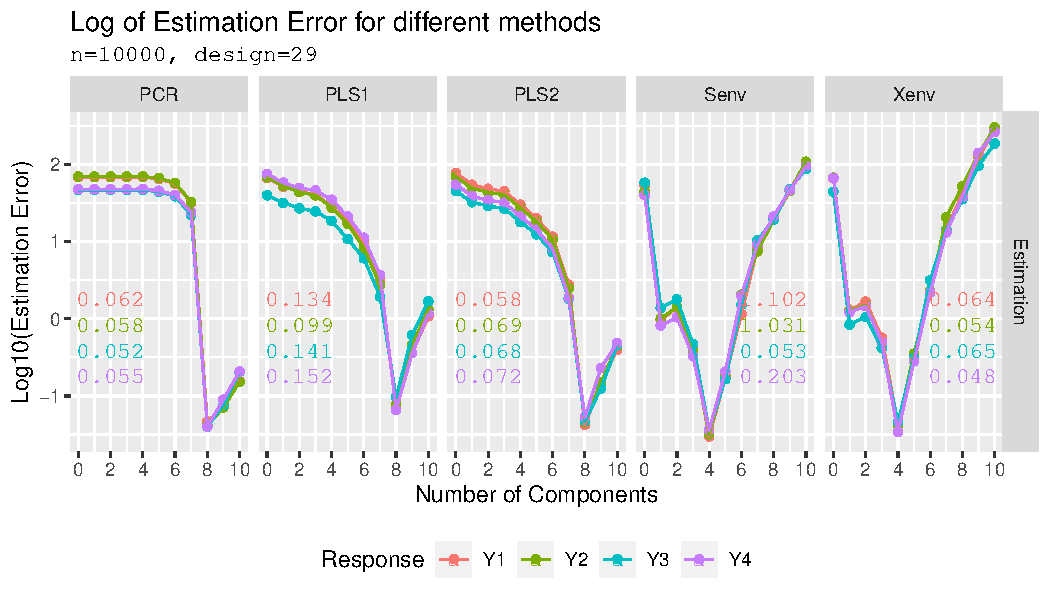
\includegraphics[width=\textwidth]{large-n-est-error.pdf}
\end{cbox}

%\pagebreak
%\nocite{*}
%\bibliographystyle{elsarticle-harv}
%\bibliography{References}

\end{document}
